\documentclass[6pt, twocolumn]{ctexart}
%\usepackage{multicol}
\usepackage{color}
\usepackage{CJK}
\usepackage{array}
\usepackage{rotating}   % 图片旋转 
\usepackage{subfigure}
\usepackage{graphicx}   % 插图必用宏包 
\usepackage{biblatex}
\usepackage{amsmath}
\usepackage{algorithmic}
\usepackage{algorithm}
\bibliography{sample}
\renewcommand{\abstractname}{摘 要}  % 将Abstract改为摘要
\renewcommand{\refname}{参考文献}   % 将References改为参考文献
\renewcommand{\indexname}{索引}
\renewcommand{\figurename}{图}
\renewcommand{\tablename}{表}
\renewcommand{\appendixname}{附录}
\begin{document}

\title{基于四种全排列生成算法的实现与优化}
\author{刘宁\footnote{刘宁 2016310624 liu-n16@mails.tsinghua.edu.cn}、  李秀星\footnote{李秀星 2016210987 lixx16@mails.tsinghua.edu.cn } 、 
钟华松\footnote{钟华松 2016210988  zhonghs16@mails.tsinghua.edu.cn} \\ 清华大学计算机科学与技术系软件所\footnote{地址:北京市海淀区清华大学东主楼 }}
\date{}
\maketitle
\begin{abstract}全排列生成问题指的是,对 $n$ 个不同的数$p_1 \sim p_n$,如何无重复无遗漏地生成这 $n$ 个数的所有全排列。 全排列的应用很广泛,然而复杂度往往过高,限制了其应用的范围。本文在对字典序法,递增进位制法,递减 进位制法和邻位对换法这四种全排列经典算法的研究基础上,优化了邻位对换法和递减进位制数法,提高了两 种算法的运行效率,同时通过实验对四种经典算法和优化后的算法进行了综合比较。对相关算法的进一步改进 和新算法的提出起到了参考的作用。
	
\end{abstract}
	

%\begin{multicols}{2}
\section{ 前言 }
组合数学是一门研究离散对象的科学,是计算 机科学的基础。所以,随着计算机的应用越来越普 遍,组合数学的研究将更加深入。其研究重点之一 在于计数。学习组合数学的基础就是排列组合。排 列是指从多个不同元素中取出几个元素按照一定顺 序排成一列的过程,排列的种类数称为排列数,用$P_{n}^m$表示。组合是指从多个不同元素中取 素组成一个集合的过程,组合的种类数称为组合数,用$C_n^m$表示。



全排列生成是指无重复无遗漏的列举出 1 到 n 的所有排列。对于全排列生成的研究有很长的一段历史,1956年,C. Tompkins 写了一篇论文介绍了一些用全排列生成算法解决问题的领域\cite{Tompkins1956Machine}。由于其算法的复杂性和多样 性已经成为组合数学和计算机领域研究的重点课题之一\cite{chenweidong}。在很多问题的求解中都会用到全排列,比 如 n 皇后问题,克莱姆法则\cite{李模刚2010全排列生成算法在克莱姆法则中的应用},求出栈顺序等。全排列生成问题经常被用作计算机课程的课程实例讲授(例如\cite{吴素萍2008全排列递归算法在算法教学中的重要性,Dijkstra1979discipline})。针对全排列的生成,前人已经提出了各种各样的算法, 典型的有字典序法,递增进位制法,递减进位制法, 邻位对换法,循环左移法,循环右移法等等。

本文针对上述提到的前四种算法进行改进和实 现。本文的工作如下:\\
\begin{itemize}
  \item 介绍了四个全排列生成算法的基本原理;
  \item 优化改进了邻位对换法和递减进位制法, 优化后的 算法平均比原算法的效率提高了接近 50\% ;
  \item 实现 并对比四种基本全排列生成算法和改进后的算法。
\end{itemize}
\section{相关工作}
\subsection{字典序法}
字典序法就是按照字典序依次求出下一个排列 的算法。这要求相邻的两个字典有尽可能长的共同 前缀,将变化限制在尽可能短的后缀上。具体方法 如下:\\
设 $P$ 是 $1\sim n$ 的一个全排列:\\
\begin{displaymath}
p=p_1p_2\cdots p_n
\end{displaymath}

\begin{enumerate}
  \item 从排列的右端开始,找出第一个比右边数字小的数字的位置$j$
  \item 找出在$p_j$右边的数字中,比$p_j$大的数中最小的数字$p_k$
  \item 交换$p_j$和$p_k$
  \item 将序列$p_{k+1}\sim p_{n}$倒转即可以得到下一个序列 
\end{enumerate}	

除此之外,字典序法也可以通过中介数进行计 算。中介数是计算排列的中介环节,它 的每一位由 原排列每个数字右侧比其小的数字个数构成。 其运 算过程为:原排列→中介数→新中介数→新排列。具体的计算过程如下:

设得到的新中介数位$a = a_1\cdots a_{n-1}$,要求的排列为$p = p_1\cdots p_n$。则$p_1 = a_1 +1$。
设$x = \{p_j \mid p_j \le y\}, 0<j<i,1<i\le n,y=a_i + 1$。若$x \ne 0$,得到新的$x$,反复进行上述操作,直到$x=0$,则有$p_i = b$,由此可以得到心排列。
\subsection{递增进位制数法}
人们通常所用的进制大多是固定进位制,如 2 进制,10 进制等。$m$位$n$进制可以表示的数字个数为 $m^n$个。而递增/递减进位制数,顾名思义,是指数 字的进制随着数字位置的不同递增/递减的进制。$m$ 位递增/递减进位制数可以表示$m!$数字。例如递增进 位制 4121,它的进制从右向左依次为 2、3、4、5, 换算成十进制相当于数字 107。

利用递增进位制数法生成下一个全排列时,需 要将原排列与下一个排列中间相隔排列的个数转换 为递增进位制数进行加减运算。

以 839647521 的下 100 个排列举例,具体步骤如下 :
\begin{enumerate}
\item 将原排列映射为中介数:按照从 9 到 2 的顺序,依次求出在原排列中每个数字右侧比它小的数 字个数,放在中介数的相应位置。得递增进位制中 介数为 67342221;
\item 由原中介数计计算出新中介数:由中介数加上 100 的递增进位制数 4020 得新中介数为 67351311;
\item 由新中介数还原成新排列:设新中介数的位置号从左到右依次为$9,8,\cdots 2,1$。对于每一个在位置 $i$ 的中介数$x$,将其放在从右到左数第$y+1$,个未被占用 的位置,在余下的最后一个空格上填入 1,产生新排 列 869427351。
\end{enumerate}
\subsection{递减进位制数法}
可以看到,递增进位制方法由于要频繁地进位, 所以算法效率受到了一定的限制。因此想到利用递 减进位制数生成全排列。其方法与递增进位制类似, 生成的中介数为递减进制中介数,恰好为递增进位 制数法得到的中介数的镜像,在此不再赘述。
\subsection{邻位对换法}
由递减进位制数法可以得到启发,通过交换相 邻两位来得到下一个排列,由此便产生了邻位对换 法。递减进位制数字的换位是单向的,从右向左, 逐个换位,直到最左端。邻位对换法的换位是双向 的,通过保存数字的“方向性”来快速得到下一个 排列,得到的中介数是递减进位制数。 具体步骤如 下:
\begin{enumerate}
	\item 初始化:初始序列为从 1 到 n 的升序序列, 每个元素的方向向左;
	\item 查找当前序列的最大可移动数$p_i$ :可移动数 该数沿着箭头方向的一侧有比其小的数;
	\item 按照箭头方向,将该可移动数$p_i$ 和其相邻的数 交换;
	\item 翻转所有大于$p_i$数的箭头方向,即可得到下 一个排列;
\end{enumerate}
邻位对换法也可以通过中介数来生成序列的全 排列。。设当前序列的中介数为$a = a_1\cdots c_{n-1}$,下一个排列为$p = p_1 \cdots p_n$,则从排列的右端到左端,依次判断$p_i$的奇偶性。若$p_i$为奇数,其方向性由$a_{i-1}$决定,奇向右、偶向左;若$p_i$为偶数,其方向性决 定于$a_{i-1}+a_{i-2}$的奇偶性,同样是奇向右、偶向左。当得到方向性后,$a_i$的值就是背向$p_i$的方向直到排列 边界这个区间里比$p_i$小的数字的个数。如此就能得 到邻位对换法的中介数,同理,可以通过中介数推 断当前序列的方向,从而得出该排列。





\section{基于中介数的求后续排列优化}
在很多应用场景下,我们需要求出某个排列后面的第$m$个排列。\textcolor{red}{比如...?}设原排列为$P$,目标排列即原排列的后续第$m$个排列为$\bar{P}$。在字典序法,递增进位制法,递减进位制法和邻位对换法中求$\bar{P}$的方法一般为首先找到原排列的中介数$A$,然后将中介数加$m$得到新的中介数$\bar{A}$,依据新的中介数找到目标排列。本节基于动态规划的思想,提出了一种优化求解中介数的算法,该算法在一般情况下可以优化一般算法$3-3.5$倍时间。
\subsection{求后续排列的一般算法}
以字典序算法为例,算法\ref{next_permutation} 给出了求目标排列的基本流程。首先通过GET\_AGENCY函数获取原排列$P$的中介数$A$,将$m$按照中介数进制(从左到右每位的进制依次是$n,n-1,...,2$)表示,得到$A_m$(第3-6行)。然后将$A$和$A_m$相加,得到$\bar{A}$(第7-17行)。最后根据新的中介数$\bar{A}$求出目标排列$\bar{P}$。
\begin{algorithm}
\caption{NEXT\_PERMUTATION (P,m,n)}
\label{next_permutation}
\begin{algorithmic}[1]
\STATE $A=$ GET\_AGENCY$(P,n)$
\STATE {$A_m,\bar{A},\bar{P} \leftarrow [0]$}
\FOR{$i \leftarrow n-1$ to $1$} 
\STATE {$A_m[i] \leftarrow m\%(n+1-i)$}
\STATE {$m \leftarrow m/(n+1-i)$}
\ENDFOR
\STATE {$flag,tmp \leftarrow 0$}
\FOR{$i \leftarrow n-1$ to $1$} 
\STATE {$tmp \leftarrow A[i]+A_m[i]+flag$}
\IF{$tmp\ge n+1-i$}
\STATE {$\bar{A}[i] \leftarrow tmp-(n+i-i)$}
\STATE {$flag \leftarrow 1$}
\ELSE
\STATE {$\bar{A}[i] \leftarrow tmp$}
\STATE {$flag \leftarrow 0$}
\ENDIF
\ENDFOR
\STATE calculate $\bar{P}$ from $\bar{A}$
\RETURN $\bar{P}$
\end{algorithmic}
\end{algorithm}



\iffalse
\begin{equation}
f(n,i) =\begin{cases}
n&if \quad i \ne 0(mod \quad n)\\
f(n-1,\lfloor \frac{i}{n} \rfloor ) & else	
\end{cases}
\end{equation}


\begin{equation}
A[I[i]]=\begin{cases}
i−1−A[I[i]]       \quad \quad  S1=S         \\
A[I[i]]        \quad   \quad \quad \quad   S2=S   \\
\begin{cases}
A[I[i+1]]+A[I[i]] \quad I[i]<I[i+1]  \\
A[I[i+1]]−A[I[i]]−1  \quad I[i]>I[i+1] \\
\end{cases}
\end{cases}
\end{equation}

\begin{equation}
A[I[i]]=\left\{
\begin{array}{ll}
i−1−A[I[i]] &  S1=S         \\
A[I[i]]     &  S2=S   \\
  \multicolumn{2}{l}{\left\{
  \begin{array}{llll}
    A[I[i+1]]+A[I[i]]   & I[i]<I[i+1]  \\
    A[I[i+1]]−A[I[i]]−1 & I[i]>I[i+1] \\
  \end{array}
  \right.}
\end{array}\right.
\end{equation}
\fi



\subsection{求中介数的一般算法}
在字典序算法中,中介数$A[i]$表示$P[i]$右边比$P[i]$小的数字的个数。算法\ref{get_agency} 给出了求解中介数的一般算法。该算法包括两层循环,外层循环遍历排列中的每一个数,内层循环找出这个数对应的中介数,即找出该数右侧比它小的数字个数。因此算法\ref{get_agency} 的时间复杂度为$O(n^2)$。当$n=100000$时,仅求解中介数就需要大约$24s$,这是十分耗费时间的。因此改进中介数的求解算法是十分必要的。

\begin{algorithm}
\caption{GET\_AGENCY (P,n)}
\label{get_agency}
\begin{algorithmic}[1]
\STATE {$A \leftarrow [0]$}
\FOR{$i \leftarrow 1$ to $n-1$} 
\FOR{$j \leftarrow i+1$ to $n$} 
\IF {$P[j]<P[i]$}
\STATE {$A[i] \leftarrow A[i]+1$}
\ENDIF
\ENDFOR
\ENDFOR
\RETURN $A$
\end{algorithmic}
\end{algorithm}



\subsection{求中介数的优化算法}
通过观察中介数的求解过程,我们得到了两个重要的结论:
\begin{enumerate}
  \item 当求解排列中某个数$i$的中介数时,设$i$左右两侧排列分别为$P1$,$P2$,若$i$左侧数字个数小于右侧数字个数,即$|P1|<|P2|$,那么扫描$P1$中比$i$小的数字个数可以更快的得到$i$的中介数;
  \item 设$i$与$i+1$之间的排列为$P3$,若已知$i+1$的中介数,且$i$与$i+1$在排列$P$中距离很小,即$|P3|<min(|P1|,|P2|)$,那么可以通过$i+1$的中介数快速求解出i的中介数;
\end{enumerate}
设$P=P[1],P[2],...,P[n]$,数组$I$存储排列中每个数的下标,即$I[P[i]]=i$。综合以上观察,在求解排列中数i的中介数时,由于$i$在$P$中的位置为$I[i]$,故$P1=P[1:I[i]]$,$P2=P[I[i]+1:n]$,$P3=P[I[i]:I[i+1]]$,令$P_{min}=min(P1,P2,P3)$,即$P1$,$P2$,$P3$中最短的一段,通过扫描$P_{min}$中比$i$小的数字个数(设为$t$)来计算$i$的中介数,即$A[I[i]]$,可以有效缩短计算中介数的时间。当$P1$最短时,$t$为$i$左侧比$i$小的数字个数,而比$i$小的数字个数共有$i-1$个,故$A[I[i]]=i-1-t$;当$P2$最短时,$A[I[i]]=t$;当$P3$最短时,若$i$位于$i+1$左侧,即$P=...,i,...,i+1,...$,由于比$i+1$小的数都会比i小,故而$i$的中介数等于$t$加上$i+1$的中介数,若$i$位于$i+1$的右侧,即$P=...,i+1,...,i,...$,则$i$的中介数等于$i+1$的中介数减去$1+t$。算法\ref{get_agency_optimization} 展示了这一过程。

\iffalse
\begin{equation}
A[I[i]]=\left\{
\begin{array}{ll}
i−1−A[I[i]] &  S1=S         \\
A[I[i]]     &  S2=S   \\
A[I[i+1]]+A[I[i]]  & S3=S  \\
\end{array}\right.
\end{equation}

\begin{equation}
A[I[i]]=\left\{
\begin{array}{ll}
i−1−A[I[i]] &  S1=S         \\
A[I[i]]     &  S2=S   \\
A[I[i+1]]−A[I[i]]−1  & S3=S  \\
\end{array}\right.
\end{equation}
\fi


\begin{algorithm}
\caption{GET\_AGENCY\_OPTIMIZATION (P,n)}
\label{get_agency_optimization}
\begin{algorithmic}[1]
\STATE calculate $I$ from $P$
\STATE calculate $A[I[n]]$
\FOR{$i \leftarrow n-1$ to $1$} 
\STATE {$P1 \leftarrow P[1:I[i]]$}
\STATE {$P2 \leftarrow P[I[i]+1:n]$}
\STATE {$P3 \leftarrow P[I[i]:I[i+1]]$}
\STATE {$P_{min} \leftarrow min(P1,P2,P3)$}
\STATE {$t \leftarrow$ the number of numbers in $P_{min}$ smaller than $i$}
\IF {$P1=P_{min}$}
\STATE {$A[I[i]] \leftarrow i-1-t$}
\ELSIF {$P2=P_{min}$}
\STATE {$A[I[i]] \leftarrow t$}
\ELSE 
\IF {$I[i]<I[i+1]$}
\STATE {$A[I[i]] \leftarrow A[I[i+1]]+t$}
\ELSE
\STATE {$A[I[i]] \leftarrow A[I[i+1]]-t-1$}
\ENDIF
\ENDIF
\ENDFOR
\RETURN $A$
\end{algorithmic}
\end{algorithm}


\subsection{优化算法性能分析}
优化算法每次扫描的排列序列为$P1$,$P2$,$P3$中最短的一段,因此从理论上来说优化算法可以有效减少求中介数的时间。而且当排列较为均匀,即$\sum_{i=1}^{n-1}\left|I[i]-I[i+1]\right|$较小时(比如$P=1,2,3,...,n$),由于$P3$很小,优化算法可以在接近$O(n)$的时间内求出排列的中介数。为了对优化算法进行性能分析,我们设计了一系列实验来进行测试。
图\ref{random_agency} 给出了求中介数一般算法和优化算法对随机生成排列的实验结果。由图可知,当$n<1000$时,GET\_AGENCY和GET\_AGENCY\_OPTIMIZATION的性能所差无几,而当$n>1000$后,优化算法大致可以加速一般算法$3-3.5$倍。
图\ref{even_agency} 给出了算法关于均匀数据的实验结果。由图可看出,优化算法对于均匀数据可以加速较多,当$n<500000$时,优化算法的运行时间小于$5ms$。

\begin{figure}
\label{agency_experiment}
\subfigure[随机数据]{
\label{random_agency}
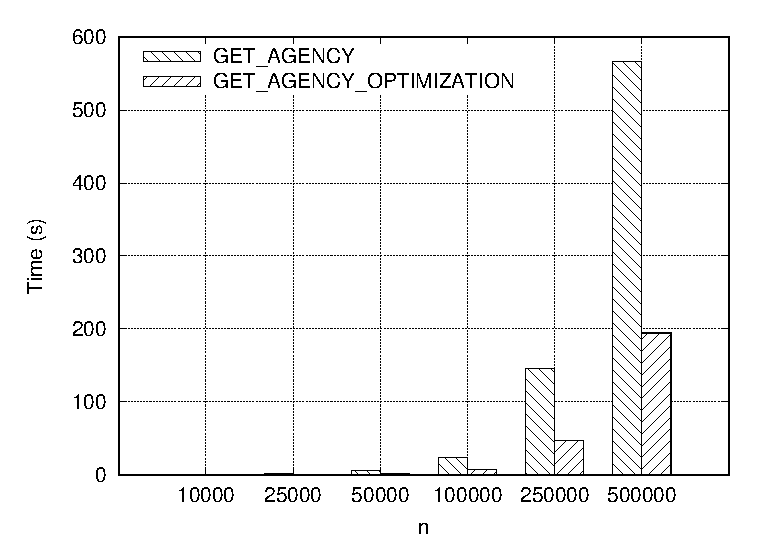
\includegraphics[width=1\columnwidth]{pictures/random_agency.eps}}
\subfigure[均匀数据]{
\label{even_agency}
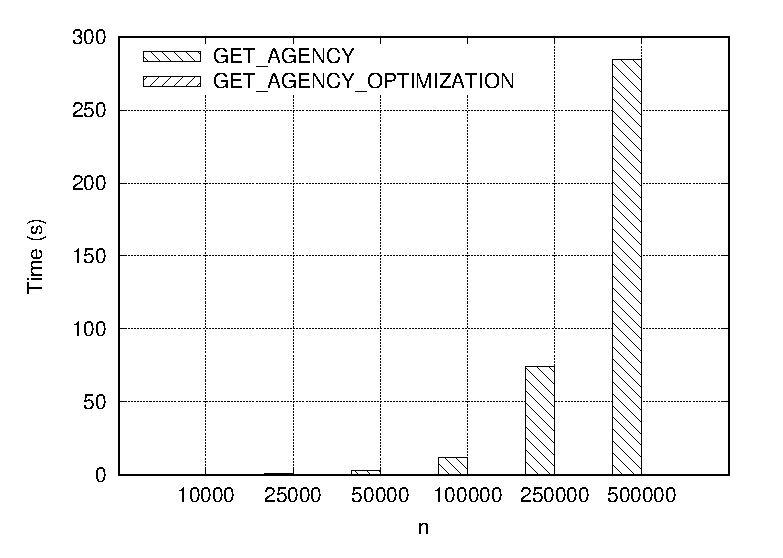
\includegraphics[width=1\columnwidth]{pictures/even_agency.eps}}
\caption{中介数优化算法性能分析}
\end{figure}







\section{基于递减进位制的一种改进}
\subsection{中介数进位规律}
根据 2.3 节的描述,递减进位制数法不会经常产生连续进位,因而依次生成全排列时,中介数的计 算有时是不必要的。而邻位对换算法通过交换相邻 两位来得到下一个排列,简单直接。综合两个算法 的优劣,发现当排列对应的递减进位制中介数不产 生连续进位时,可以直接交换排列的相邻两位。而 当递减进位制中介数连续进位时,中介数右端数字 都变成了0,因而排列之间也有规律可循。所以,本 文对递减进位制数法提出一种不用计算出中介数的 改进方法:
\begin{algorithm}
\caption{DECREASE\_IMPROVEMENT ( p,n)}
\label{alg2}
\begin{algorithmic}[1]
\PRINT p
\FOR{$i \leftarrow 1$ to $n$}
\STATE find the first $i$ where $p[i] \ne n+1-i$
\IF{$i > n$}
\RETURN permutation generation end
\ENDIF
\FOR{$j \leftarrow i+1$ to $n$}
\STATE find first $j$ where $p[j] = n+1 -i$
\ENDFOR
\STATE \textbf{swap} $p[j]$,$p[j-1]$
\FOR{$k \leftarrow i$ to $n$ }
\STATE {$p[k-i+1] \leftarrow p[k]$}
\ENDFOR
\FOR{$r \leftarrow n-i+2$ to $n$}
\STATE {$p[r] \leftarrow r$}
\ENDFOR
\ENDFOR
\end{algorithmic}
\end{algorithm}

假设$P$是$1 \sim n$的一个全排列,$p = p_1 \cdots p_n$ ,对应的中介数为$a = a_1 \cdots a_{n-1}$,若从$p = 1,2 \cdot n$开始生成全排列,则初始时中介数$𝑎 = 0$,由于$a_{n-1}$ 对应 的是数字 $n$ 右侧比 $n$ 小的数字的个数,所以$a_{n-1}$ 连 续加 1 不会立刻产生进位。因此,$p$ 中只有 $n$ 对应 的中介数相应的位数加 1,也就是排列 p 中位于 n 右边的比 n 小的数的个数加 1。这时,其他数的相对 位置不变,所以只需将 n 连续地与其左边的数交换 位置,直到$p_1=n$。

当$p_1 =n$时,排列数对应的中介数加 1 会产生 进 位 。假 设 此 时 的 中 介 数 为$a = a_1 \cdots a_{n-1}$,连续进位位数为 2 , 即$a_{n-1}=n-1,a_{n-2}=n-2 ,a_{n-3}<n-3$,所以$a_{n-3}^{'}=a_{n-3}+1$,,也就是$n − 2$右侧多了一个比它小的数,对应到排列中,就是$n − 2$和它左边的数交换 了位置。所以,需要在排列 $p$ 中找到连续下降序列 最后一位的数字 $x$,假设其在位置 $j$,然后找到比它 小 1 的数 $y$,与其左边数交换,再把连续下降序列翻 转放在排列末尾即可。

由原排列求出相邻的下一个排列的算法伪代码(DECREASE\_IMPROVEMENT $( p,n)$)。

以 1,2,3,4 的全排列举例,其全排列生成过程如下:$1 2 3 4 → 1 2 4 3 → 1 4 2 3 → 4 1 2 3 → 1 3 2 4 → 1 4 2 3 → …→ 4 3 2 1$。其中,生成 $1 2 3 4 → 1 2 4 3 → 1 4 2 3 →4 1 2 3$ 的过程中,中介数不进位,4 依次 与前面的数交换位置,而 $4 1 2 3 → 1 3 2 4$ 的生成过 程中,3 与 2 交换位置,4 插入排列尾部。之后的生 成一直重复这一过程。
\subsection{优化算法复杂度分析}
由上述的分析可知,当$p+1\ne n$ 的时候,要进行 置换得到新的排列,复杂度为$O(n)$,而已知全排列 个数为$n!$,所以外层循环的复杂度为$O(n!)$,进而可 得算法复杂度为$O(n * n!)$,相比递减进位制$O(n^2*n!)$的复杂度提高了一个数量级。
\section{实验}
本文在 4G 内存,Intel(R) Core(TM) i5-4200M 处 理器,2.50GHZ 主频,64 位操作系统的笔记本电脑 上进行实验。
\subsection{基于邻位对换法的对比}
本节主要对比以下三种算法:

\emph{基于蛮力法的邻位对换}:该方法采用邻位对换 法的基本思想,在查询最大可移动数时, 从大到小 遍历当前排列中的元素,直到找见某个元素,该元 素满足沿着该元素的箭头方向有小于该元素的数。

\emph{基于维护数组的邻位对换}:该方法在蛮力法的 基础上,增加一个长度为n的数组leftlittle来 有元素的左边比其小的元素个数。则比元素i小并位 于其右侧的元素个数为$i-1-leftlittle[i]$。该数组需 要在交换排列中元素的时候分情况修改。

\emph{基于公式的邻位对换}:该方法使用公式(1)求解 最大可移动数。
\begin{figure}
\centering	

\caption{邻位对换法算法比较图}
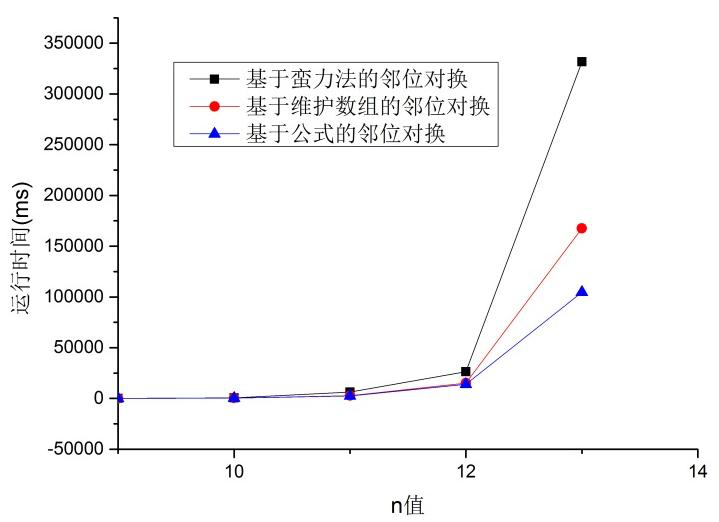
\includegraphics[width=7cm, height=4cm]{1.png}	
\end{figure}

通过图1 可知,在 $n$ 值一定的情况下,基于 蛮力法的邻位对换算法运行最慢,其次是基于维护 数组的邻位对换,效果最好的是基于公式的邻位对换算法。基于公式的邻位对换算法在 n 值越大的情 况下效果越明显。相比于原算法,优化后的算法运 行时间降低了将近一半,运行效率提高了 50\%。
\subsection{基于递减进位制法的对比}

本节主要对比一下两种算法:

\emph{递减进位制数法}:该方法采用递减进位制中介 数,先计算当前排列的递减进位制中介数,再计算 出新的中介数,进而推断出新排列。

\emph{优化的递减进位制法}:该方法利用了递减进制 中介数的进位规律,通过交换原排列中相应元素的 位置,在不计算中介数的前提下,推出下一个排列。
\begin{figure}
\centering	

\caption{递减进位制算法比较}
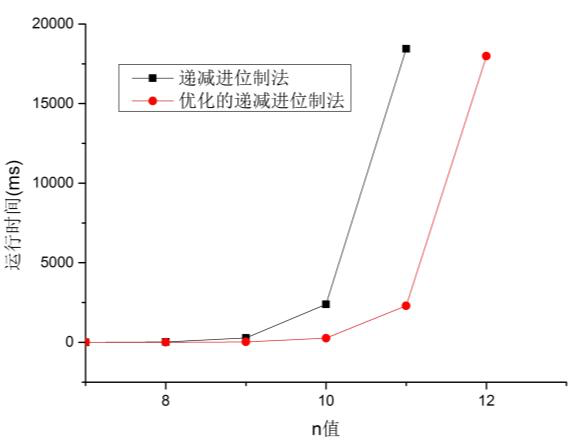
\includegraphics[width=7cm, height=4cm]{2.png}	
\end{figure}
由图2 可见,当 n 值较小时,两种方法的运 行时间差别不明显。而当 n 值大于等于 10 时,优化 的递减进位制法的运行时间明显小于原算法。这是 因为改进算法只需对排列元素进行一遍操作,便能 找出下一个排列,所以相较于原算法,运行时间降 低了一个数量级。


\subsection{四种基本全排列算法及两种优化算法的对比}
我们将上文提到的两种改进算法和第一部分提 到的四种基本算法进行对比,分析比较得出各种算 法的优缺点,并给出下一步优化方案。

\begin{figure}
\centering	

\caption{四种基本全排列算法及两种优化算法的比较}
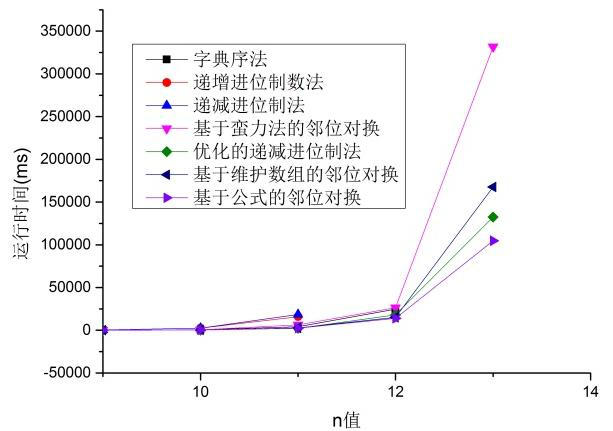
\includegraphics[width=7cm, height=4cm]{3.png}	
\end{figure}
如图3 所示,本文提到的七种算法效果最好 的是基于公式的邻位对换法,其次是优化的递减进 位制法。其中在 n=12 时,递减进位制法和递增进位 制法已不能在规定时间内运行完毕,而字典序法的 瓶颈在n = 13。可见在求全排列的过程中递减进位 制法和递增进位制法效率较低,主要原因是上述两 种算法通过中介数列举全排列,导致转化过程较为 复杂。
\section{总结与展望}
本文深入研究了全排列的四种经典算法,字典 序法,递增进位制数法,递减进位制法和邻位对换 法,并对比了其算法效率。根据邻位对换法最大可 移动数的规律,在查找最大可移动数的算法上进行 了优化 , 以提高查找 最大 可移动数的效率。 将原$O(n^2*n!)$的复杂度降为$O(n* n!)$,在 n 值固定的情况 下,运行时间降低了 50\%。同时,通过观察递减进 位制数法排列和中介数的规律,对其进行改进,使 其时间复杂度由$O(n^2*n!)$优化到了$O(n * n!)$。当 n 相 对较小时,算法有着明显的时间效率优势。



综上所述,本文实现并比较了四种全排列生成 算法,并对邻位对换法和递减进位制法进行了初步 的优化。然而,本文所实现的优化算法还不够完美, 例如递减进位制改进算法,当 n 相对较小时,算法 优化程度明显提高,但随着 n 的增大,算法的时间 优势不再明显。如何从本质上进一步提高全排列生 成算法的效率,是下一步需要考虑的问题。
\printbibliography
%\end{multicols}


\end{document}
